%---------------------------------------------------------------
\chapter{Contribution}\label{chapter:contribution}
%---------------------------------------------------------------

This is the main chapter of the thesis.
On this place, we present our contribution to the topic of the \HL problem.
We first review a proof of a theorem about \HLdeg from Waniek et al. \cite{Waniek2017} and show
its correctness for our definition of \HL.
Then, we present our own proofs for \HLdeg regarding various parameters and complexity classes.
Lastly, we put our results in the context of the work of other authors,
visualizing the parameterized complexity results for \HLdeg discovered both by us and by authors
from the literature.


%---------------------------------------------------------------
\section{Proof revision}\label{section:proofRevision}

Waniek et al. \cite{Waniek2017} proposed three hardness results for the \HL problem given degree, closeness and betweenness
centralities. In this section, we review the first aforementioned result with respect to our definition of \HLshort.
The original theorem reads: \emph{``The \HL problem is \NPc given the degree centrality.''}.
The proof adjustments are pretty straightforward but to better understand them,
let us first briefly describe the idea of that proof.

A common way of proving \NP-hardness is to propose a polynomial reduction from another \NPh problem to the
problem we are proving \NP-hardness of.
In this proof, the authors show a reduction from the $k$-\textsc{Clique} problem defined on graph $G$.
The idea is following: In a polynomial time, construct a new graph $H$ from $G$ in a way that
in order to solve \HL in $H$ we must solve $k$-\textsc{Clique} in $G$ in the first place.
To achieve that, the authors, as a starting point of $H$, first create a complement of $G$ 
where all vertices are marked as followers. This will be the only followers in final $H$.
This initial construction assures that every possible solution of \HLshort will only consists of edges from $G$, that is,
$W \subseteq E(G)$ (and $F' \subseteq V(G)$).
Next, they add two types of leaders into $H$, each type with a different purpose.
Leaders of the first type act like ``regularizators'' as their only job is to connect with followers (in some way) and,
by doing so, make degree of every follower the same and equal to $n$.
These leaders are denoted as $X$ and $y$ in the original proof.
The task of the second type, having no connection with followers at all,
is then to set a maximum degree across all leaders, which followers from $F'$ will have to reach.
These leaders are denoted as $L'$ and are practically the only concern of our adjustments to which we now proceed.

We allow equality of centralities between followers from $F'$ and leaders in our definition of \HL.
To compensate it, we just need to create one extra leader of the second type, that is,
$|L'| = n+k$ as opposed of $|L'| = n+k-1$ in the original proof,
leading to all leaders from $L'$ having degree of $n+k-1$, as opposed of $n+k-2$ in the original proof.
Now note that this is the highest degree among the leaders and that all the followers have degree $n$,
so, in order to be part of $F'$, they must obtain at least $(n+k-1) - n = k-1$ new neighbors.
We got into exactly the same situation as in the original proof and since, as stated above,
leaders from $L'$ do not have any other purpose than setting the maximum degree of all leaders,
the rest of the arguments presented in the proof remain unchanged.

We have just shown that allowing equality of centralities between followers from $F'$ and leaders does not
break the proof presented by Waniek et al. \cite{Waniek2017}.
The other change in our definition of \HL is that we allow all members to be leaders, $L = V$,
but since such instances are trivial as they are $yes$-instances if and only if $d = 0$,
there is nothing to change in the proof.


%---------------------------------------------------------------
\section{Our results}\label{section:OurResults}

The next proof is built on the same idea Waniek et al. \cite{Waniek2017} presented in their proof of
\NP-completeness of \HLshort for the degree centrality measure.
We reviewed the proof from Waniek et al. and its core ideas in Section \ref{section:proofRevision}.
We present a proof of a stronger theorem, with simpler reduction graph and in the language of parameterized complexity.
These results are possible mainly because of a stronger assumption in the proof where we assume a regular graph as the input.

The core idea of the proof is that we construct a network in such way that finding a solution $W$ of the \HL problem
correspond to finding a solution of the problem we started with, essentially having the starting network
present in the constructed network in some manner and then finding a solution inside of it.

\begin{theorem}\label{theorem:DB}
    \HL parameterized by $b + d$ is \Wh even if $|L| = 1$.
\end{theorem}

\begin{proof}\label{proofDB}
    To proof this theorem, we propose a parameterized reduction from the $k$-\textsc{Clique} problem on regular graphs,
    which is known to be \Wh with respect to $k$ \cite{Mathieson2008}.
    
    Suppose we have a parameterized $k$-\textsc{Clique} instance $(G, k)$, where $|V(G)|=n$, $G$ is a $r$-regular graph and $n-2 \geq r \geq k \geq 3$
    (for $r > n-2$ or $r < k$ or $k < 3$ the problem is trivial).
    Then, we construct a graph $H$ in the following way:
    \begin{enumerate}
        \item Start with an empty graph $H$.
        \item Add all vertices from $G$, \emph{i.e.}, $V(H) \leftarrow V(G)$, mark these vertices as $F_1$.
        \item Add all edges from $\overline{G}$, \emph{i.e.}, $E(H) \leftarrow E(\overline{G})$.
        \item Add an extra vertex $\ell$, \emph{i.e.}, $V(H) \leftarrow V(H) \cup \{\ell\}$.
        \item Add an edge between vertex $\ell$ and $n - r + (k - 1) = \lambda$ arbitrarily chosen vertices $X \subset F_1$,
        \emph{i.e.}, $E(H) \leftarrow E(H) \cup \{ (\ell, x) \mid x \in X \}$.
        \item For each vertex $v \in V(H) \setminus X \eqqcolon Y$, introduce a new vertex $w_v$ and add edge $\{v, w_v\}$, \emph{i.e.},
              $V(H) \leftarrow V(H) \cup \{ w_v \mid v \in Y \}$ and $E(H) \leftarrow E(H) \cup \{ (v, w_v) \mid v \in Y \}$,
              mark the set of $w_v$ for each $v \in Y$ as $F_2$.
    \end{enumerate}
    An example of such construction can be seen in Figure \ref{fig:proofDB}.

    Note that step 5 can always be done because $r \ge k$, so $|F_1| = n > n - r + (k - 1)$
    and since $deg(l) = 0$ (before step 5), there are enough vertices for $\ell$ to connect with.
    Considering $G$ is $r$-regular, its complement, constructed and added into $H$ in steps 2 and 3, must be $(n-r-1)$-regular.
    After connecting all the $F_1$ vertices either with $\ell$, or the corresponding $w_v$ in steps 5 and 6,
    they all end up with degree $n-r$; in other words, graph $H[F_1]$ is $(n-r)$-regular.
    Also note that the construction of $H$ is done in time polynomial to $n$.
    Now we show how finding a $k$-clique in graph $G$ corresponds to finding a solution $W$ of \HLshort in $H$.

    Let us take $\mathcal{I} = (H, \{\ell\}, \frac{k\cdot(k-1)}{2}, c, k)$, where $c$ is a degree centrality measure,
    as an instance of \HLdeg with $k' \coloneqq b + d = \frac{k\cdot(k-1)}{2} + k$ as a parameter.
    First we note that degree of the only leader $\ell$ is $\lambda$, as presented above.
    The other vertices $V(H) - l$ are naturally followers of which we can recognize two types, $F_1$ and $F_2$,
    where $\forall_{f_1 \in F_1} deg(f_1)$ = $n-r$ and $\forall_{f_2 \in F_2} deg(f_2)$ = $1$.
    Whereas $F_1$ are vertices of the original graph $G$,
    $F_2$ plays a role of ``partners'' of vertices $Y$, since their only job is to substitute a missing connection with $\ell$.

    Because we just have one leader in $\mathcal{I}$, it is clear that for any follower $f' \in F'$ applies that
    $deg(f') \geq \lambda = n - r + (k - 1)$.
    Also, because $n > r$, $\max\limits_{\forall f_1 \in F_1}deg(f_1) = n-r > 1 = \max\limits_{\forall f_2 \in F_2}deg(f_2)$.
    With this in mind, we state the following:

    \begin{lemma}\label{lemmaInProof}
        No $F'$ can contain vertex from $F_2$, i.e., $F' \cap F_2 = \emptyset$.
    \end{lemma}
    \begin{subproof}
        Assume $F' \subseteq F_1$. This is a valid assumption because $|F_1| = n > k$ and it must be at least $d = k$ vertices in $F'$.
        Because all vertices from $F_1$ have degree $n-r$, we must have added at least $\lambda - (n - r) = k - 1$ new neighbors to all vertices from $F'$.
        Since the budget $b$ in $\mathcal{I}$ is $\frac{k\cdot(k-1)}{2}$,
        the only possible way of how $F'$ could have been constructed is that $|F'|=k$ and the newly added edges $W \subset F_1 \times F_1$, $|W| = b$
        connect all the $k$ vertices $f' \in F'$ in a way that graph $(F', W)$ forms a $k$-clique.
        From this and from the statements above, we can see that no vertex from $F_2$ can be in $F'$
        since there will never be large enough budget $b$ to let us reach the safety margin $d$.
    \end{subproof}

    As shown in the proof of Lemma \ref{lemmaInProof}, every feasible solution $W$ of \HLshort for instance $\mathcal{I}$, together with corresponding $F'$,
    will form a $k$-clique.
    Note that every edge from $W$ must be an edge from the original graph $G$ because $W \subset F_1 \times F_1$ and $F_1 = E(G)$
    and also all the edges from $E(\overline{G})$ are already in $E(H)$ so they cannot be in $W$ since it only contains newly added edges.

    Because a solution $W$ for \HLshort in $H$ exists if and only if a $k$-clique in $G$ exists,
    we can conclude that finding a solution for the \HL problem in graph $H$ is exactly the same as
    finding a solution for the $k$-\textsc{Clique} problem in graph $G$.

    The reduction presented in this proof is a valid parameterized reduction because;
    $(G, k)$ is a yes-instance of the $k$-\textsc{Clique} problem if and only if $\mathcal{I}$ is a yes-instance of \HLdeg;
    the construction of $H$ is done in time polynomial to $n$;
    and there is a function of $k$, $g(k) = \frac{k\cdot(k-1)}{2} + k$, upper-bounding the parameter $k'$ of $\mathcal{I}$.
\end{proof}

% Figure - proof 1
\begin{figure}[t!]
    \centering
    % G
    \begin{subfigure}[t]{.46\textwidth}
        \centering
        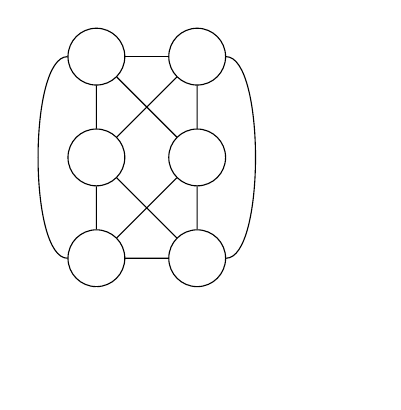
\begin{tikzpicture}[node distance={16mm}, scale=0.8, every node/.style={scale=0.8}]
            \tikzstyle{vertex} = [circle, draw=black, text=white]
            \tikzstyle{edge} = []
            
            \node[vertex] (g1) at (0,0) {$f_{1_1}$};
            \node[vertex] (g2) [right of = g1] {$f_{1_2}$};
            \node[vertex] (g3) [below of = g1] {$f_{1_3}$};
            \node[vertex] (g4) [right of = g3] {$f_{1_4}$};
            \node[vertex] (g5) [below of = g3] {$f_{1_5}$};
            \node[vertex] (g6) [right of = g5] {$f_{1_6}$};
            \draw[edge] (g1)--(g2);
            \draw[edge] (g5)--(g6);
            \draw[edge] (g1)--(g3);
            \draw[edge] (g3)--(g5);
            \draw[edge] (g2)--(g4);
            \draw[edge] (g4)--(g6);
            \draw[edge] (g3)--(g2);
            \draw[edge] (g3)--(g6);
            \draw[edge] (g4)--(g1);
            \draw[edge] (g4)--(g5);
            \draw[edge] (g1) to [out=180,in=180,looseness=0.5] (g5);
            \draw[edge] (g2) to [out=0,in=0,looseness=0.5] (g6);
            % dummy to ensure the same height as the other subfig
            \node (l) [right of = g4] {};
            \draw[color=white] (l) to [out=315,in=270] (g5);
        \end{tikzpicture}
        \caption{
            ~A $4$-regular ($r = 4$) graph $G$ with $n=6$ vertices,
            playing a role of the input graph for the $k$-\textsc{Clique} problem and
            is the starting point of our construction.
        }
    \end{subfigure}%
    ~~~~
    % H
    \begin{subfigure}[t]{.46\textwidth}
        \centering
        \begin{tikzpicture}[node distance={16mm}, scale=0.8, every node/.style={scale=0.8}]
            \tikzstyle{followerG} = [circle, draw=black]
            \tikzstyle{edgeG} = [dashed, draw=green!40, thick]

            \tikzstyle{edgeCompl} = []

            \tikzstyle{followerF2} = [circle, fill=red!50]
            \tikzstyle{edgeF2} = [draw=red!50]

            \tikzstyle{square} = [regular polygon, regular polygon sides=4]
            \tikzstyle{leader} = [square, fill=blue!50, label={[text=blue!50]above:$\ell$}]
            \tikzstyle{edgel} = [color=blue!50]

            % G in H
            \node[followerG] (g1) at (0,0) {$f_{1_1}$};
            \node[followerG] (g2) [right of = g1] {$f_{1_2}$};
            \node[followerG] (g3) [below of = g1] {$f_{1_3}$};
            \node[followerG] (g4) [right of = g3] {$f_{1_4}$};
            \node[followerG] (g5) [below of = g3] {$f_{1_5}$};
            \node[followerG] (g6) [right of = g5] {$f_{1_6}$};
            \draw[edgeG] (g1)--(g2);
            \draw[edgeG] (g5)--(g6);
            \draw[edgeG] (g1)--(g3);
            \draw[edgeG] (g3)--(g5);
            \draw[edgeG] (g2)--(g4);
            \draw[edgeG] (g4)--(g6);
            \draw[edgeG] (g3)--(g2);
            \draw[edgeG] (g3)--(g6);
            \draw[edgeG] (g4)--(g1);
            \draw[edgeG] (g4)--(g5);
            \draw[edgeG] (g1) to [out=180,in=180,looseness=0.5] (g5);
            \draw[edgeG] (g2) to [out=0,in=0,looseness=0.5] (g6);
            % complement
            \draw[edgeCompl] (g1)--(g6);
            \draw[edgeCompl] (g2)--(g5);
            \draw[edgeCompl] (g3)--(g4);
            % leader
            \node[leader] (l) [right of = g4] {};
            \draw[edgel] (l)--(g4);
            \draw[edgel] (l)--(g6);
            \draw[edgel] (l) to [out=45,in=90] (g1);
            \draw[edgel] (l) to [out=315,in=270] (g5);
            % partners
            \node[followerF2, label={[text=red!50]above:$f_{2_1}$}] (f2) [above of = g2] {};
            \node[followerF2, label={[text=red!50]above:$f_{2_2}$}] (f3) [left of = g3] {};
            \draw[edgeF2] (f2)--(g2);
            \draw[edgeF2] (f3)--(g3);
        \end{tikzpicture}
        \caption{
            ~A graph $H$ constructed from graph $G$ where $H[F_1]$ is $2$-regular.
            The black vertices are followers from $F_1$,
            the red vertices are followers from $F_2$ and
            the blue vertex is leader.
            The black edges are edges $E(\overline{G})$ and the green, dashed lines represent edges from $G$,
            which are not present in $H$, but from which a potential solution $W$ of \HLshort would be picked.
        }
    \end{subfigure}
    \caption{A sample construction of graph $H$ as presented in Proof \ref{proofDB}.}
    \label{fig:proofDB}
\end{figure}


% Corollaries
We have just shown that \HL parameterized by $b+d$ is \Wh even with a constant number of leaders.
We can easily see that \HLshort remains \Wh even when parameterized by $|L|+b+d$.
This is because the problem is \Wh already for $|L|$ bounded by a constant function,
hence, bounding it by a nonconstant function will not make the problem easier to solve, leaving it \Wh.

\begin{remark}\label{cor:LnBD:Wh}
    \HL parameterized by $|L|+b+d$ is \Wh.
\end{remark}

Following the argument, we can see that \HL is \Wh for any variation of parameters $|L|$, $b$, $d$.
For example, if we ommit $b$ from the parameter, then $b$ is no longer bounded by a function of the parameter and
become bounded by a function of the input size, making the problem possibly harder and so leaving it \Wh.

\begin{corollary}\label{cor:LnBD:variation:Wh}
    \HL parameterized by any variation of $|L|$, $b$, $d$ is \Wh.
\end{corollary}

By taking $|L|$ as the only parameter, we get the last corollary.

\begin{corollary}\label{cor:Ln:pNPh}
    \HL is \pNPh with respect to $|L|$.
\end{corollary}


% XP algo for param d
We now look at the problem from the opposite end.
Let us remind that we interpret \W-hardness as an evidence that given problem is not in \FPT.
Hence, there is no use of trying to find FTP algorithms for \HL parameterized by $|L|$, $b$, $d$, or any of their variation.
However, there is still a chance for XP algorithms.
We now show that there are indeed such algorithms for parameters $b$ and $d$, meaning that
\HL parameterized whether by budget $b$ or by safety margin $d$ belongs to \XP.
From this we then show that \HLshort is in \XP even for the other parameter variations.
Let us present a proof of the variant with parameter $d$ first.

\begin{theorem}\label{theorem:D:XP}
    \HL parameterized by $d$ is XP.
\end{theorem}

\begin{proof}\label{proof:XPd}
    Given parameterized instance $(\mathcal{I}, d)$, where $\mathcal{I} = (G, L, b, c, d)$ is a \HLdeg instance and $d$ is the parameter,
    we show an algorithm which decides whether or not $(\mathcal{I}, d)$ is a $yes$-instance in time bounded by
    $f(d) \cdot |(\mathcal{I}, d)|^{g(d)}$ for some computable functions $f,g$.

    We start by picking gradually each of the $\binom{|F|}{d} = \Theta(|V(G)|^d)$ $d$-element subsets of followers $F$,
    we denote the current subset as $D$ and a set of edges that can be added between followers from $D$
    as $\hat{A}_D \subseteq \hat{A}$, $\hat{A}_D = E(\overline{G[D]})$.
    Because we take all the possible $d$-element subsets of $F$, we eventually find a subset $D$ such that,
    after addition of new edges, $D = F'$,
    if such $F'$ exists, that is, if $(\mathcal{I}, d)$ is a $yes$-instance.
    Then, we try to add $min(|\hat{A}_D|, b) \coloneqq t$ edges between followers from $D$ in each of the $\binom{d}{t} \leq 2^d$ possible ways.
    Note that $t$ can be $b$ because we are not allowed to add more than $b$ edges into $G$.
    From now, only these three situations can occur:

    First, we added $t$ edges into $G$ and all $D$ vertices have degree greater than $\lambda$.
    Because $|D| = d$, $(\mathcal{I}, d)$ is a $yes$-instance.
    We can check this in time $\mathcal{O}(|V(G)|)$.
    
    Second, we added $t$ edges into $G$ but not all $D$ vertices have degree greater than $\lambda$.
    Moreover, $|\hat{A}_D| < b$ and thus we know that $G[D]$ is (after adding new edges) already a complete graph
    but we still can add some edges into $G$ before reaching the budget $b$. 
    In this situation $D = F'$ if and only if there is at least $min_{\delta \in D}\{deg(\delta)\}$ followers
    outside of $D$ and a number of edges we are still allowed to add before reaching budget $b$, $b - |\hat{A}_D|$,
    is smaller than the sum of connections needed to reach $\lambda$ of all vertices from $D$,
    $\sum_{\delta \in D} min(0, \lambda - deg(\delta))$.
    This is true because in order for instance $(\mathcal{I}, d)$ to be a $yes$-instance, we must
    ensure that each follower from $D$ has degree at least $\lambda$, for what we connect them to some followers
    outside $D$ (becuase $D$ is already complete), for which there must be enough followers outside $D$ and
    we must have enough edges left before reaching $b$.
    Note that if $D = F'$, then $(\mathcal{I}, d)$ in a $yes$-instance.
    
    Third, we added $t$ edges into $G$ but not all $D$ vertices have degree greater than $\lambda$.
    Moreover, $|\hat{A}_D| \geq b$ so $t = b$ and $D \neq F'$.
    We can check this in time $\mathcal{O}(|V(G)|)$.

    Situation other than one of the three cannot occur.
    If instance $(\mathcal{I}, d)$ is not identified as a $yes$-instance for any choice of $D$,
    then we conclude that $(\mathcal{I}, d)$ is a $no$-instance because if it was a $yes$-instance,
    then we would have found it by the procedure above.
    
    The algorithm we have just described runs in time $f(d) \cdot |(\mathcal{I}, d)|^{g(d)}$ for $f(d) = 2^d$ and $g(d) = d$
    and where the instance size $|(\mathcal{I}, d)|$ is measured as $|V(G)|$.
    From this we can conclude that \HL parameterized by $d$ is XP.
\end{proof}

Notice that although the just presented algorithm is not possibly the best one we could find,
there surely cannot be so much faster algorithm since, as we already know,
there can be no FPT algorithm for \HL parameterized by $d$.


% XP algo for param b
Now we proceed to a proof of the variant with parameter $b$.
This proof will be led in a similar manner as the previous proof.

\begin{theorem}\label{theorem:B:XP}
    \HL parameterized by $b$ is XP.
\end{theorem}

\begin{proof}
    Given parameterized problem $(\mathcal{I}, b)$, where $\mathcal{I} = (G, L, b, c, d)$ is a \HLdeg instance and $b$ is the parameter,
    we show an algorithm which decides whether or not $(\mathcal{I}, b)$ is a $yes$-instance in time bounded by
    $f(b) \cdot |(\mathcal{I}, b)|^{g(b)}$ for some computable functions $f,g$.

    We start by picking gradually each of the $\binom{|\hat{A}|}{b} = \Theta(|E(G)|^b)$ $b$-element subsets of
    edges we can add between followers, we denote the current subset as $B$.
    Because we take all the possible $b$-element subsets of $\hat{A}$, if $(\mathcal{I}, b)$ is a $yes$-instance and
    thus such $W$ exists, we eventually find a subset $B$ such that $B = W$.
    Then, we try to add those $B$ edges into $G$ and after each such addition, we check whether there are at least $d$ followers
    with degree greater than $\lambda$. The addition can be done in time $b$, the check can be done in time $|V(G)|$.

    If instance $(\mathcal{I}, b)$ is not identified as a $yes$-instance for any choice of $B$,
    then we conclude that $(\mathcal{I}, b)$ is a $no$-instance because if it was a $yes$-instance,
    then we would have found it by the procedure above.

    The algorithm we have just described runs in time $f(b) \cdot |(\mathcal{I}, b)|^{g(b)}$ for $f(b) = g(b) = b$
    and where the instance size $|(\mathcal{I}, b)|$ is measured as $|E(G)| + |V(G)|$.
    From this we can conclude that \HL parameterized by $b$ is XP.
\end{proof}

We have just shown that \HL parameterized by $b$ or $d$ is XP.
If we now add some other parameter or parameters to either $b$ or $d$, then the problem
might become easier but surely stays in \XP.
For example take $b+|L|$ as the parameter;
when not a part of the parameter, |L| was bounded by a function of an input size,
because it is now a part of the parameter, |L| is bounded by a function of the parameter,
hence the problem is possibly easier to solve.
From this we get the following.

\begin{corollary}\label{cor:BD:variation:XP}
    \HL is in \XP when parameterized by at least $b$ or $d$.
\end{corollary}

Last, following the same logic and considering the results from Dey and Medya \cite{Dey2019} presented in Subsection \ref{subsection:ResultsDegree},
we can state the following.

\begin{corollary}\label{cor:Ld:variation:FPT}
    \HL is in \FPT when parameterized by at least $\lambda$.
\end{corollary}

%---------------------------------------------------------------
\section{Overview}

In this last section, we visualize the results for \HLdeg presented in Section \ref{section:OurResults},
together with the result for parameter $\lambda$ presented in Subsection \ref{subsection:ResultsDegree}.
The visualization can be seen in Figure \ref{fig:complexityPicture}.

% Figure - overview
\begin{figure}[t]
    \centering
    \begin{tikzpicture}[node distance=18mm]
        \tikzstyle{every node} = [minimum height=0.7cm,minimum width=0.9cm,scale=1.3];
        \tikzstyle{result} = [draw, very thick];
        \tikzstyle{corollary} = [draw,dashed];
        \tikzstyle{pNPh} = [fill=red!30];
        \tikzstyle{Wh} = [fill=orange!30];
        \tikzstyle{XP} = [fill=green!30];

        \tikzstyle{edgeXP} = [color=orange,-{Stealth[length=3mm]}]
        \tikzstyle{edgeW} = [color=violet,-{Stealth[length=3mm]}]
        \tikzstyle{edgeFPT} = [color=green,-{Stealth[length=3mm]}]

        % pairs
        \node[corollary,Wh,label={0:\small{\tt C\ref{cor:LnBD:variation:Wh}}}] (LnB) at (0,0) {\leadnum, \budget};
        \node[corollary,Wh,label={0:\small{\tt C\ref{cor:LnBD:variation:Wh}}}] (LnD) [right =of LnB] {\leadnum, \safetymarg};
        \node[corollary,Wh,label={0:\small{\tt C\ref{cor:LnBD:variation:Wh}}}] (BD) [right=of LnD] {\budget, \safetymarg};
        % singletons
        \node[result,Wh,label={0:\small{\tt T\ref{theorem:B:XP}}}] (B) [above left=18mm and 2mm of LnD] {\budget};
        \node[result,Wh,label={0:\small{\tt T\ref{theorem:D:XP}}}] (D) [above right=18mm and 2mm of LnD] {\safetymarg};
        \node[corollary,pNPh,label={0:\small{\tt C\ref{cor:Ln:pNPh}}}] (Ln) [left=of B] {\leadnum};
        \node[XP,label={0:\small{\tt B\cite{Dey2019}}}] (Ld) [right=of D] {\leaddeg};
        % triplets
        \node[result,Wh,label={0:\small{\tt T\ref{theorem:DB}}}] (LnBD) [below=of LnD] {\leadnum, \budget, \safetymarg};
        % edges
        \draw[->,edgeXP] (B.225) -- (LnB.135);
        \draw[->,edgeXP] (D.225) -- (LnD.135);
        \draw[->,edgeXP] (D.225) -- (BD.135);    
        \draw[->,edgeXP] (BD.225) -- (LnBD.135);
        
        \draw[->,edgeW] (LnBD.45) -- (LnB.315);
        \draw[->,edgeW] (LnBD.45) -- (LnD.315);
        \draw[->,edgeW] (LnBD.45) -- (BD.315);
        \draw[->,edgeW] (BD.45) -- (B.315);
        \draw[->,edgeW] (BD.45) -- (D.315);
    \end{tikzpicture}
    \caption
    [Overviewing graph with results for \HLdeg]
    {
        The complexity picture for the \HL problem given the degree centrality measure, \HLdeg.
        Combinations of parameters which give rise to XP algorithms are highlighted in green,
        while combinations for which \HLdeg is \Wh but still in \XP are highlighted in orange and \pNP combinations
        are highlighted in red.
        Results explicitly proved in this work are represented by a black solid border,
        their corollaries are represented by a black dashed border and
        results from the literature does not have any border.
        Each node have a reference to the corresponding theorem, remark, corollary or bibliography record.
        Arrows represent how complexity results spread.
        Green arrows represent \FPT class, orange arrows represent \XP class
        and violet arrows represent \W-hardness.
        When multiple arrows would aim to the same node, then only one a only that for the best complexity class is displayed.  
    }
    \label{fig:complexityPicture}
\end{figure}
%---------------------------------------------------------------
